\documentclass{article}
\usepackage[utf8]{inputenc}
\usepackage{amsmath}
\usepackage{amsfonts}
\usepackage{amssymb}
\usepackage{graphicx}
\usepackage{geometry}
\usepackage{xcolor}
\usepackage{gensymb}
\usepackage{hyperref}
\usepackage{gensymb}
\usepackage{listings}

\newcommand{\inv}{^{-1}}   
\newcommand{\Z}{\mathbb Z}
\newcommand{\R}{\mathbb R}
\newcommand{\Q}{\mathbb Q}
\newcommand{\C}{\mathbb C}
\newcommand{\N}{\mathbb N}

\begin{document}

\medskip\noindent\textbf{1.}

	\textbf{(a)} The voltage drop across the 5M$\Omega$ resistor is 5V, because $9 - \frac{4}{4+5} \cdot 9 = 5$.

	\textbf{(b)} The DMM and 5M$\Omega$ resistor in parallel have resistance equivalent to a single $3.33$M$\Omega$ resistor. Thus, the voltage drop across the 4M$\Omega$ resistor is $\frac4{4+3.33}\cdot9 = 4.909091$, so the voltage drop across the 5M$\Omega$ resistor is $9 - 4.909091 = 4.090909$V. Thus, the meter will display 4.09V.

\newpage\noindent\textbf{2.}

    \begin{center}
        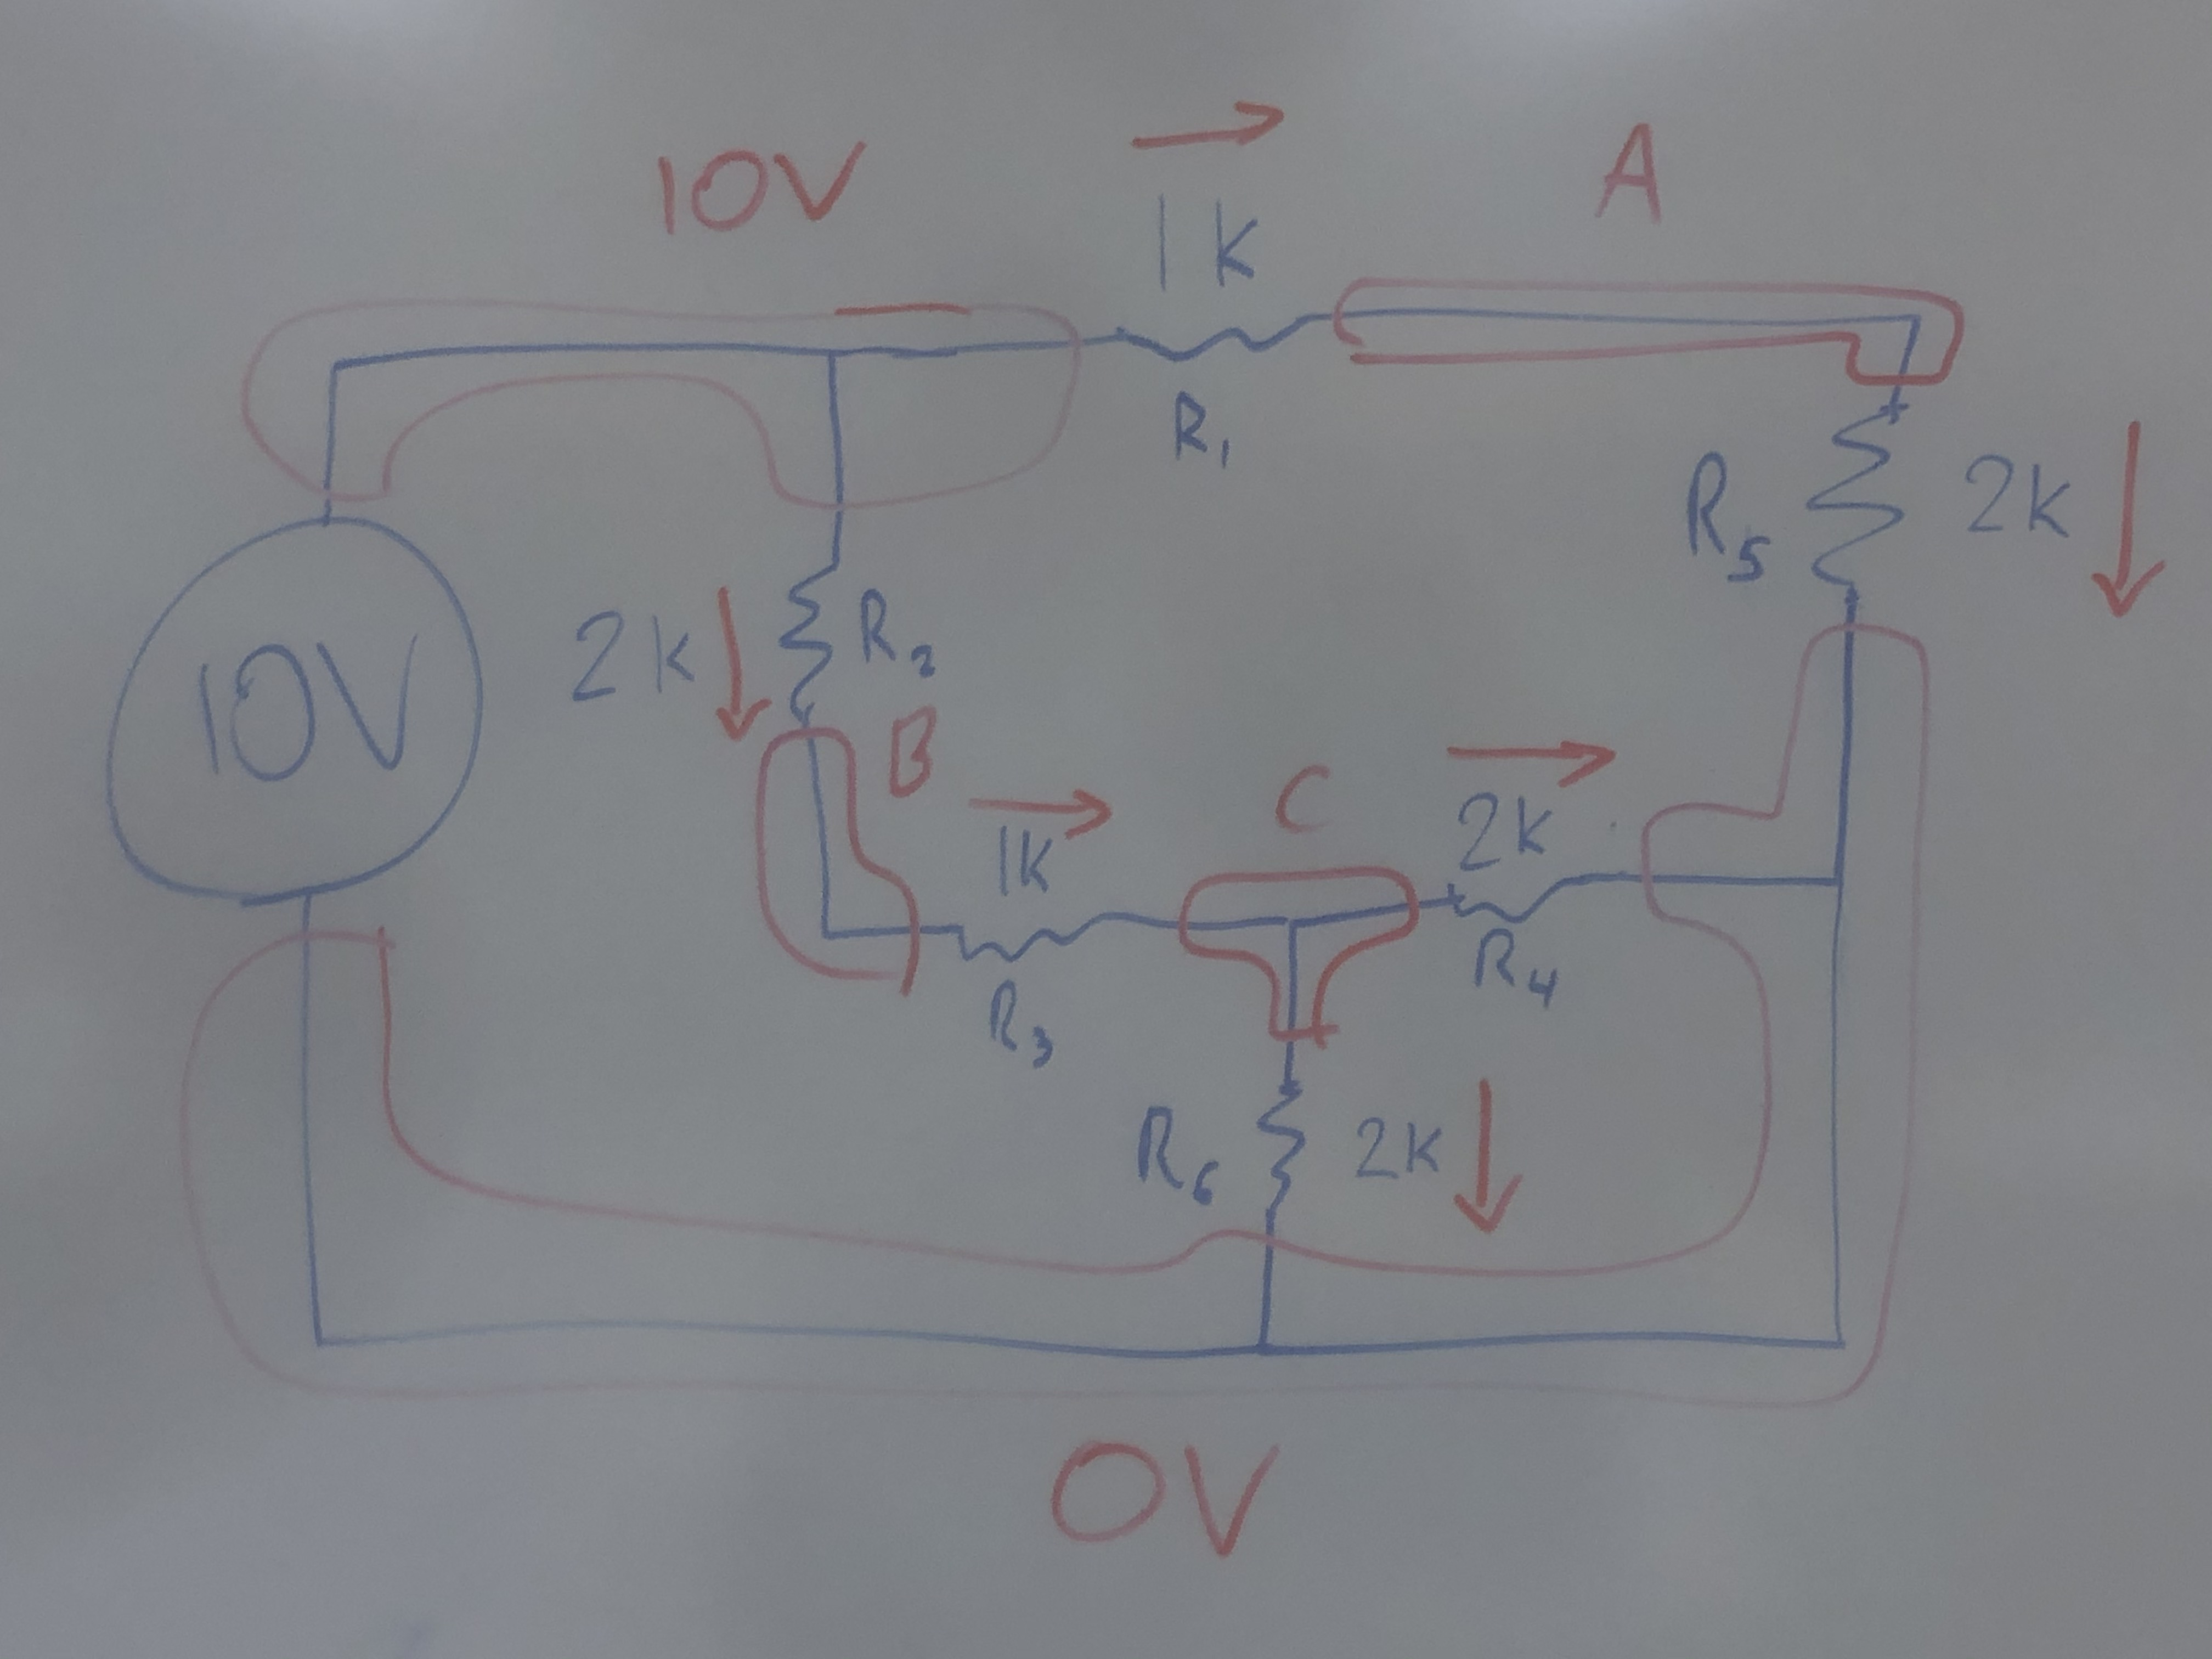
\includegraphics[scale=.07]{IMG_0869.jpg}

        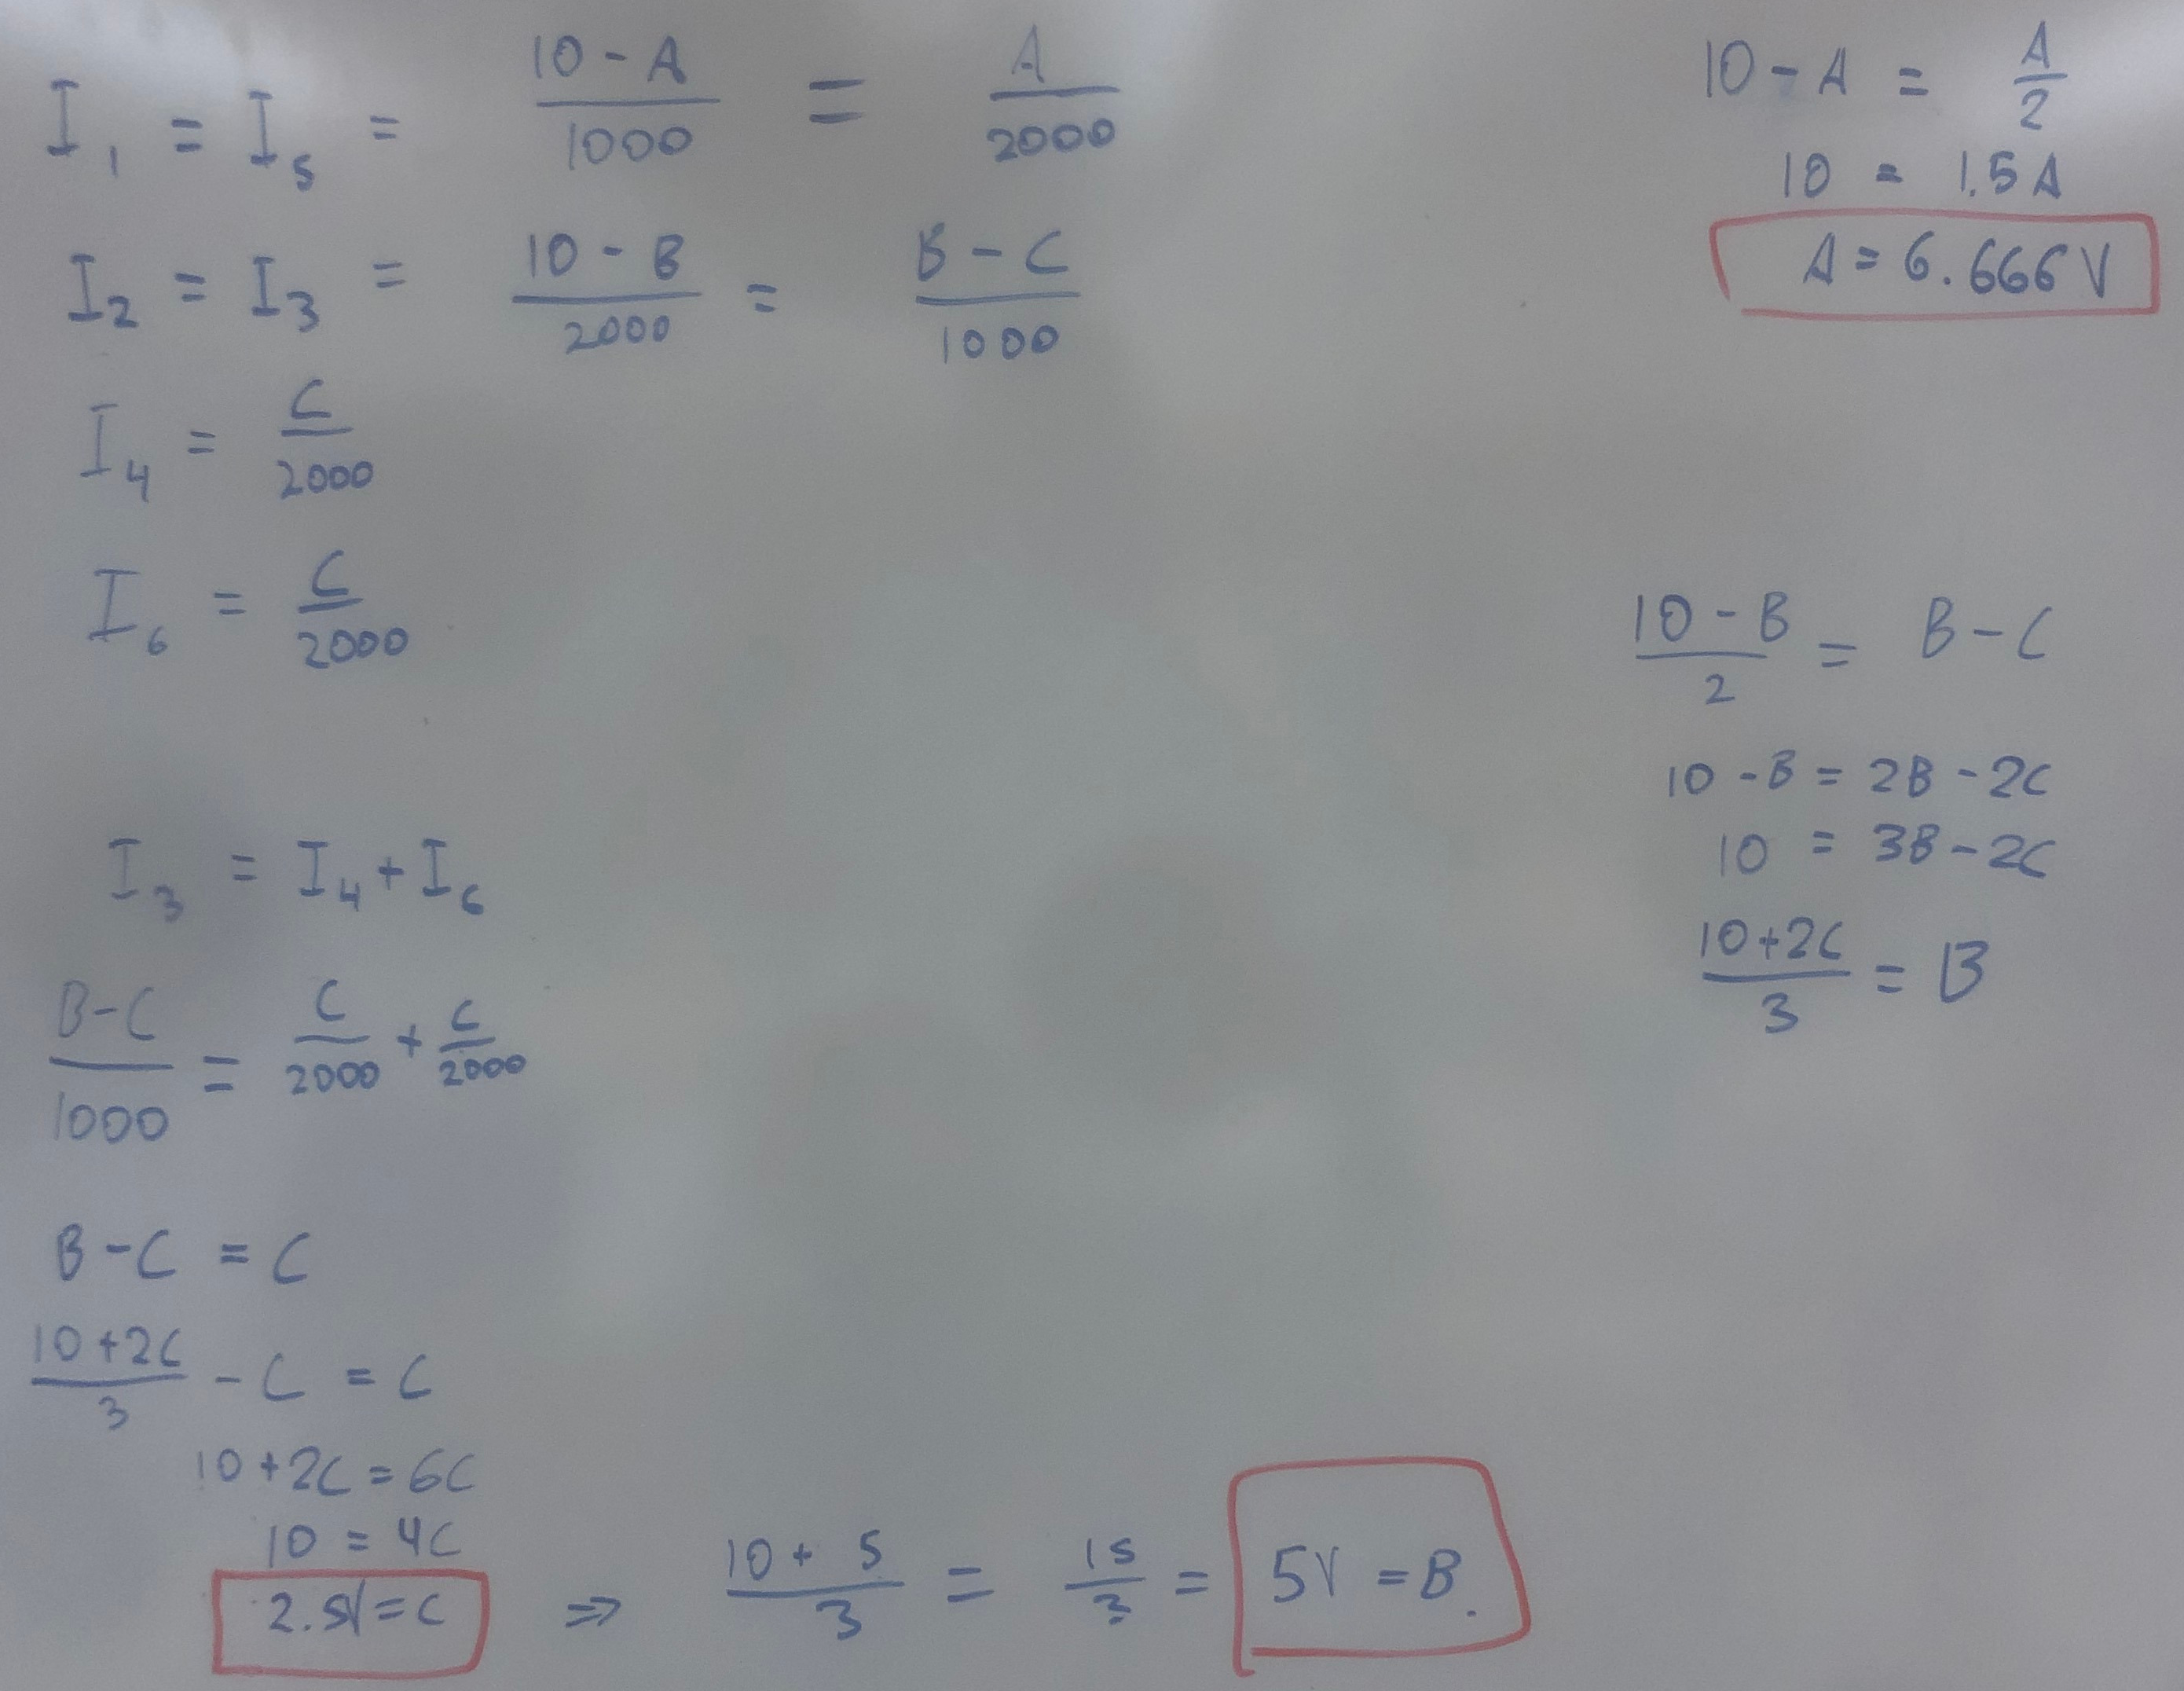
\includegraphics[scale=.1]{IMG_0870.jpg}
        
        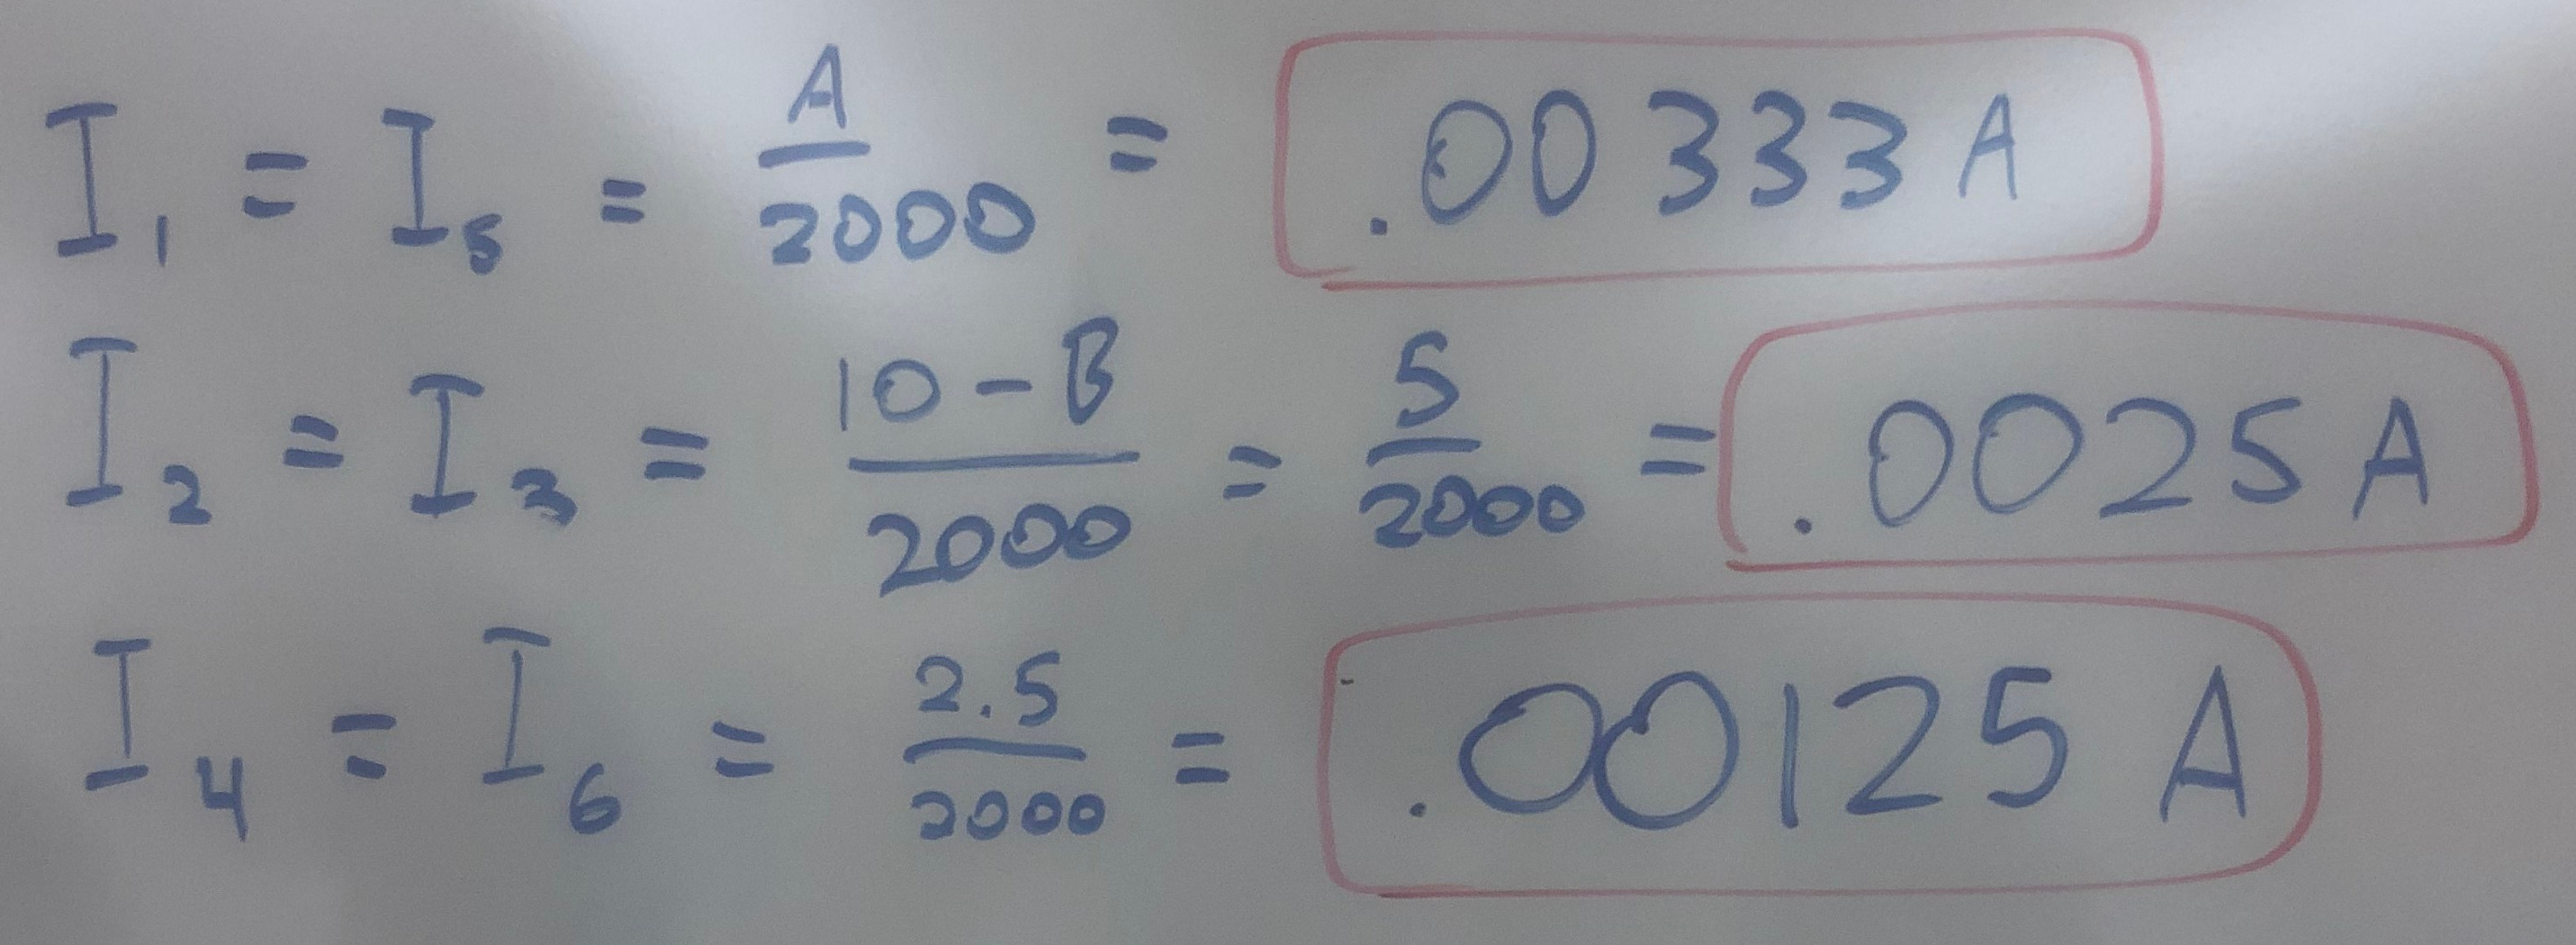
\includegraphics[scale=.1]{IMG_0871.jpg}
    \end{center}

\newpage\noindent\textbf{3.}

    The two resistors on the right are in series, so they are equivalent to a single 2k resistor.
    That 2k resistor is parallel with another 2k resistor, so they are equivalent to a single 1k resistor.
    That 1k resistor is in series with another 1k resistor, so they are equivalent to a single 2k resistor.
    Thus, the circuit has resistance 2k$\Omega$.

\newpage\noindent\textbf{4.}

	When both switches are open, Vout is 5V. When one or both switches are closed, Vout is 4.4V, because there needs to be a voltage drop of .6V across any diode participating in the circuit.

\newpage\noindent\textbf{5.}

	Based on the circuit diagram of NOR given on page 12-16, and the circuit diagram of NOT given on page 12-1, this circuit computes
	\begin{align*}
		!A \text{ NOR } !B &= !(!A \text{ OR } !B) \\
				 &= !(!(A \text{ AND } B)) \\
				 &= A \text{ AND } B.
	\end{align*}

\newpage\noindent\textbf{6.}

    \begin{center} 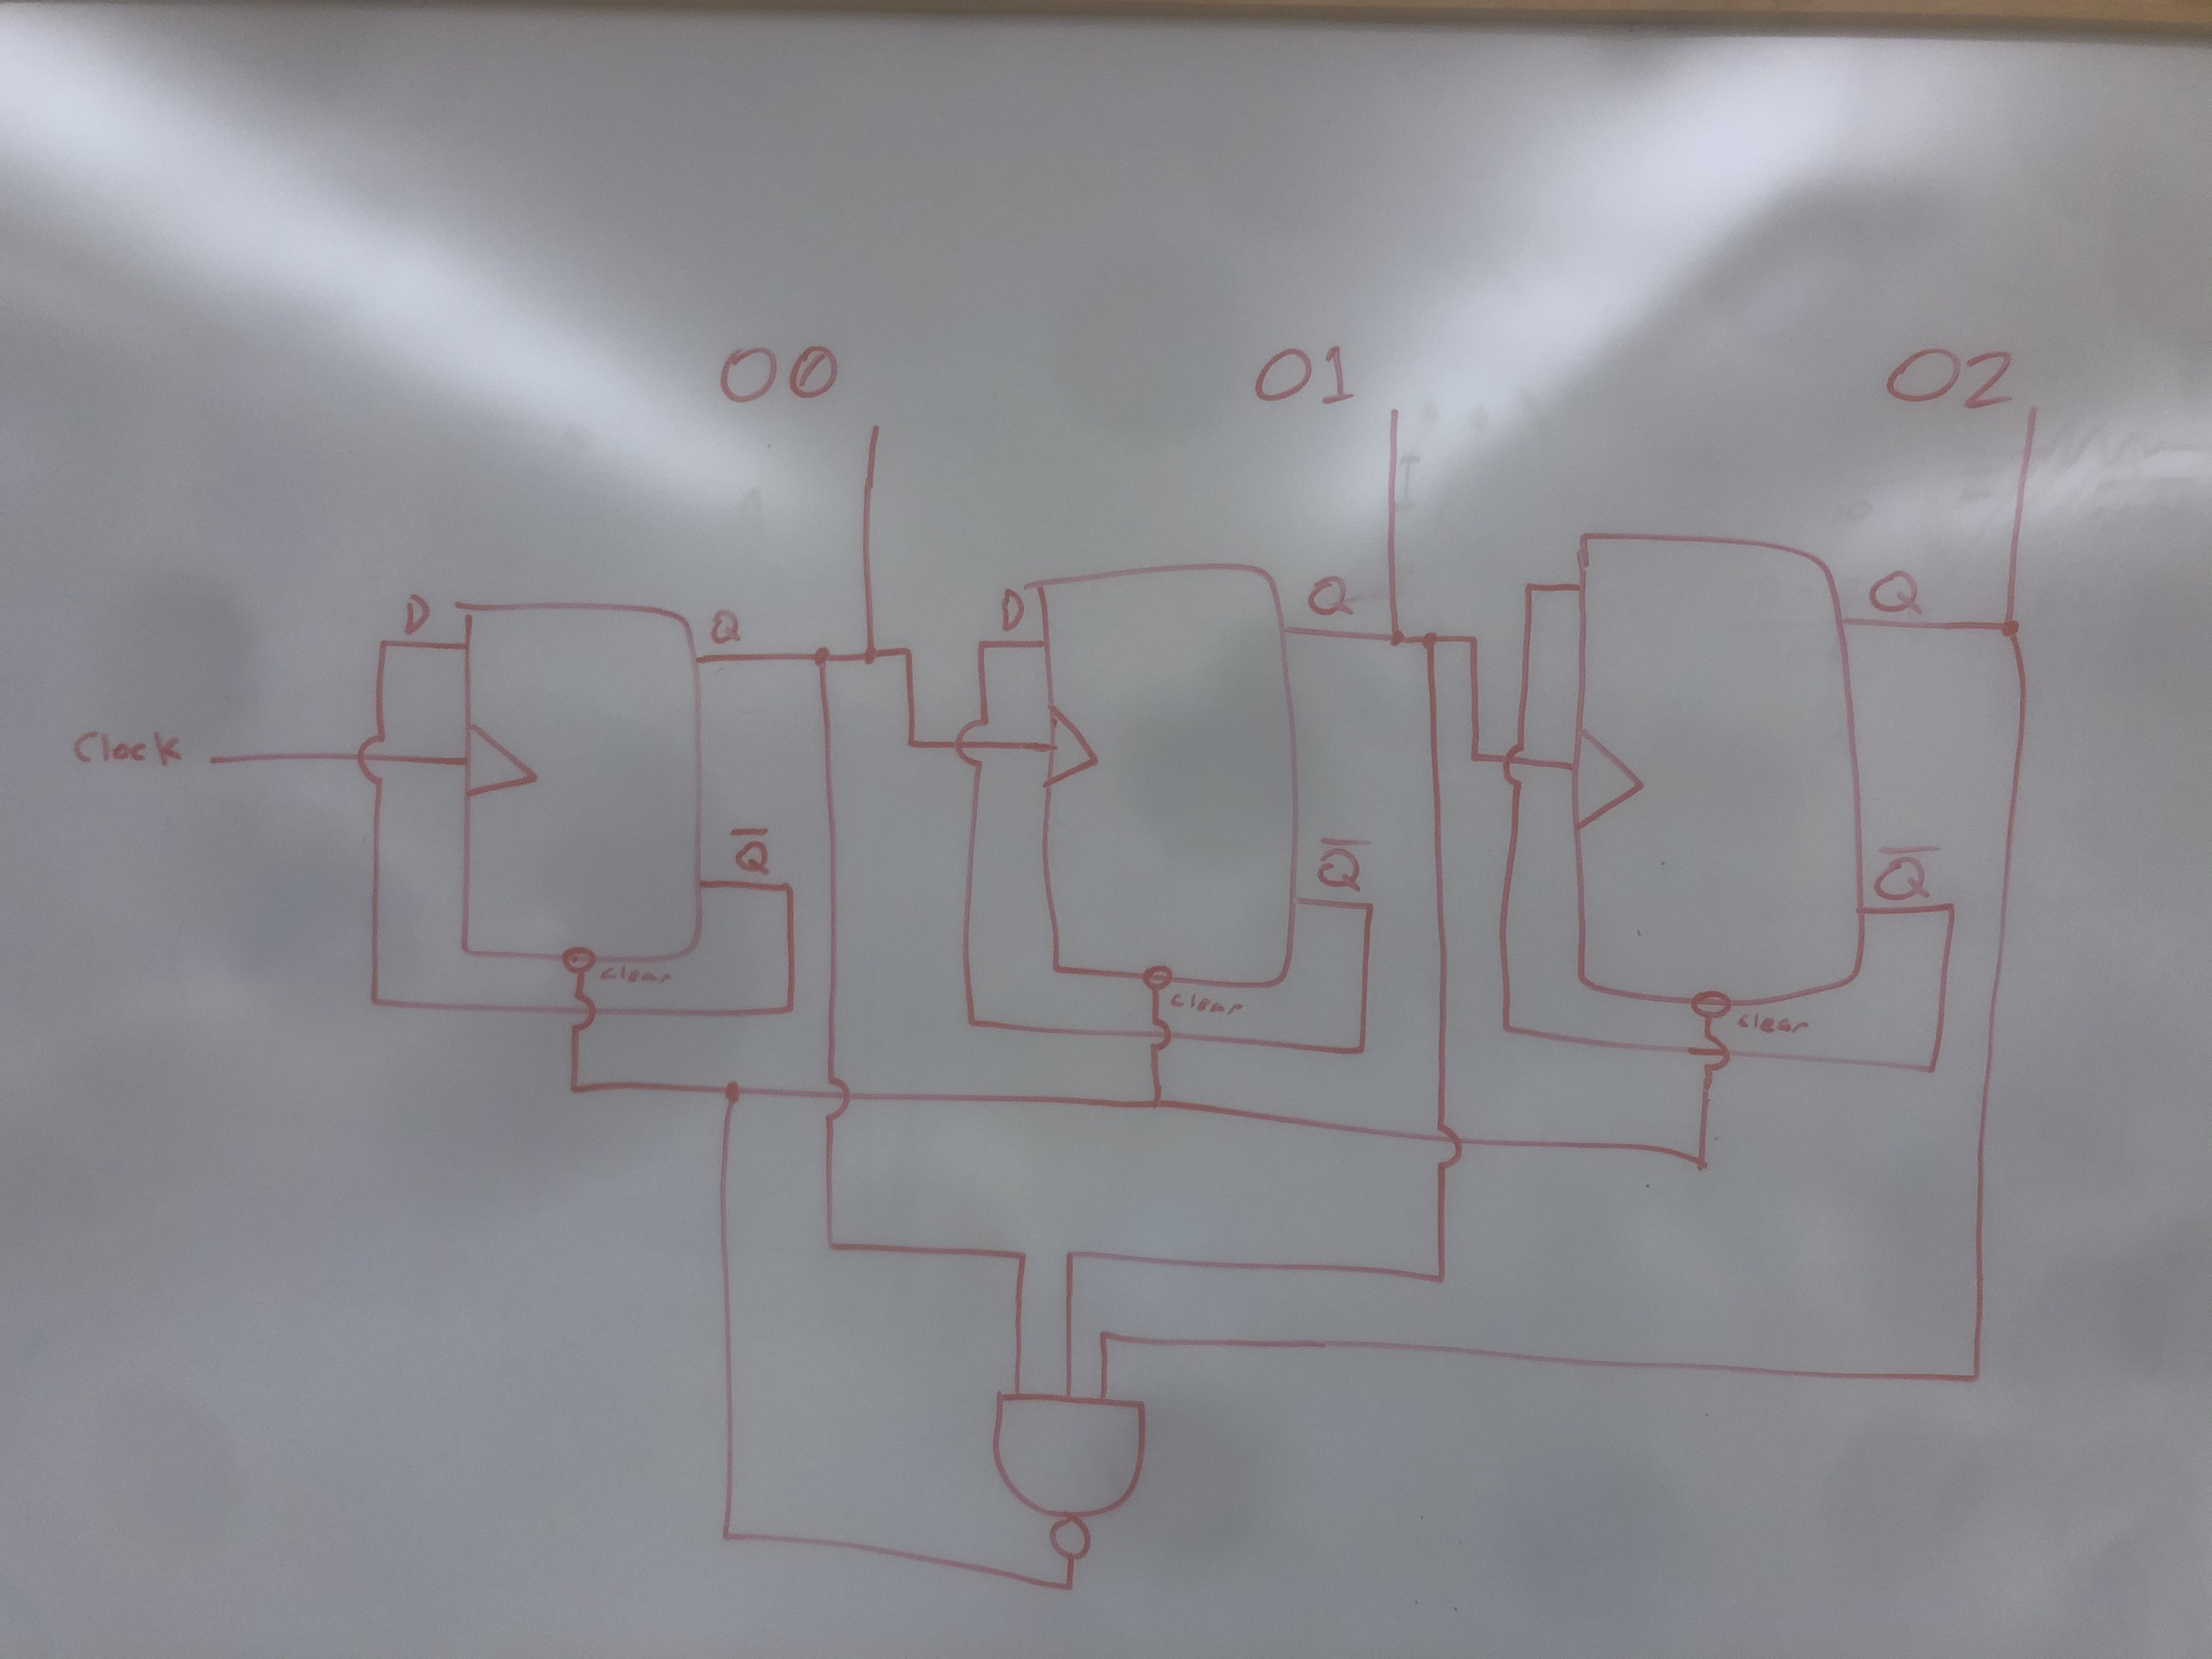
\includegraphics[scale=.1]{IMG_0872.jpg} \end{center}

\newpage\noindent\textbf{7.}

	Figure 16.1 cannot be represented with logical equations because the output of the 1-1 state is impossible to determine without knowing the prior state of the circuit.

\newpage\noindent\textbf{8.}

    \begin{center}
        0.01$\mu$F
        
        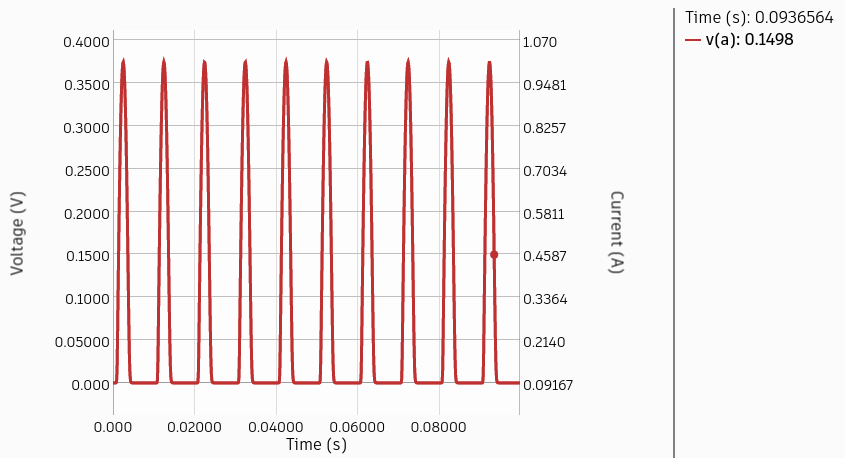
\includegraphics[scale=.4]{81.png}

        \medskip

        1$\mu$F

        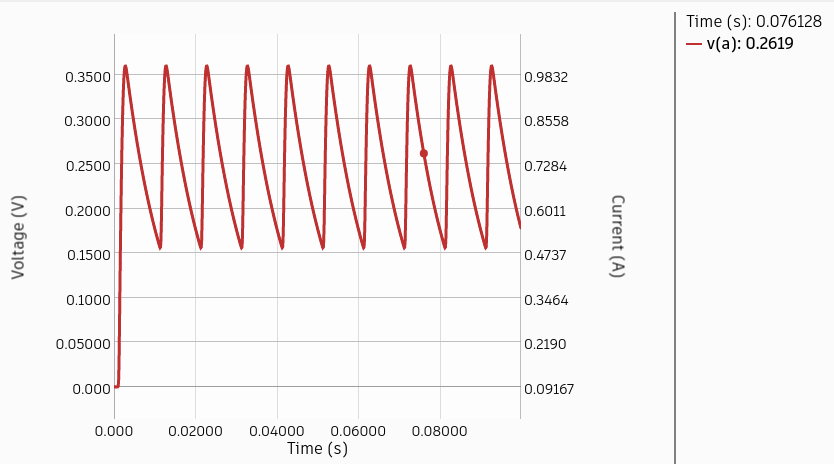
\includegraphics[scale=.4]{810.png}

        \medskip

        100$\mu$F

        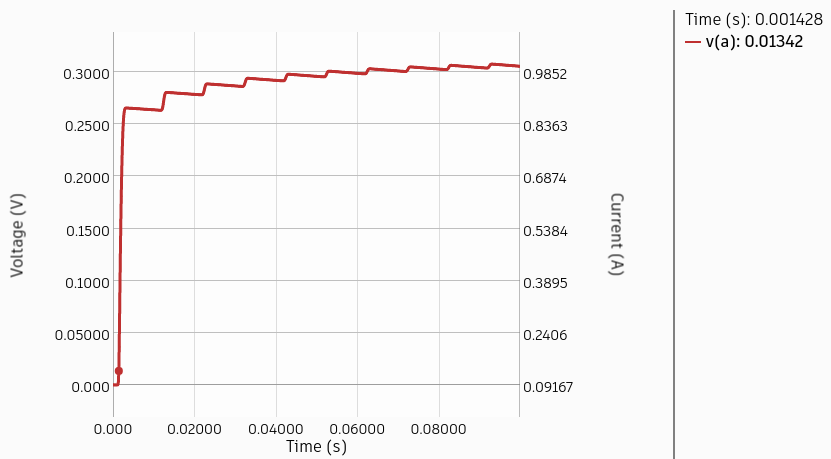
\includegraphics[scale=.4]{8100.png}
    \end{center}

    The diode prevents the lower half of the sine wave from reaching the resistor and the capacitor. Thus, the input wave will look like the top half a sine wave.
    With a 0.01$\mu$F capacitor, the capacitor is able to fully discharge for each period of the input wave. Thus, we see many thin peaks in the output, similar to having no capacitor at all.
    With a 1$\mu$F capacitor, the capacitor is able to partially discharge for each period of the input wave, so the voltage at point $a$ never reaches 0.
    WIth a $100\mu$F capacitor, the capacitor discharges very little of its totally capacity during each period of the input wave. Thus, we see the voltage at point $a$ approach the peak voltage of the input wave.

\newpage\noindent\textbf{9.}

    \begin{tabular}{| c | c | c | c | c |}
        \hline
        A & B & C & D & OUT \\
        \hline
        0 & 0 & 0 & 0 & 1 \\
        0 & 0 & 0 & 1 & 0 \\
        0 & 0 & 1 & 0 & 0 \\
        0 & 0 & 1 & 1 & 1 \\
        0 & 1 & 0 & 0 & 0 \\
        0 & 1 & 0 & 1 & 1 \\
        0 & 1 & 1 & 0 & 1 \\
        0 & 1 & 1 & 1 & 0 \\
        1 & 0 & 0 & 0 & 0 \\
        1 & 0 & 0 & 1 & 1 \\
        1 & 0 & 1 & 0 & 1 \\
        1 & 0 & 1 & 1 & 0 \\
        1 & 1 & 0 & 0 & 1 \\
        1 & 1 & 0 & 1 & 0 \\
        1 & 1 & 1 & 0 & 0 \\
        1 & 1 & 1 & 1 & 1 \\
        \hline
    \end{tabular}

    \medskip The output is true for even parity.

\newpage\noindent\textbf{10.}

	\begin{verbatim}def pulse(pin, period, on_time):
	    while True:
	        pin.value = 1
	        time.sleep(on_time)
	        pin.value = 0
	        time.sleep(period - on_time)
	\end{verbatim}

\end{document}
